\begin{figure}[ht!]
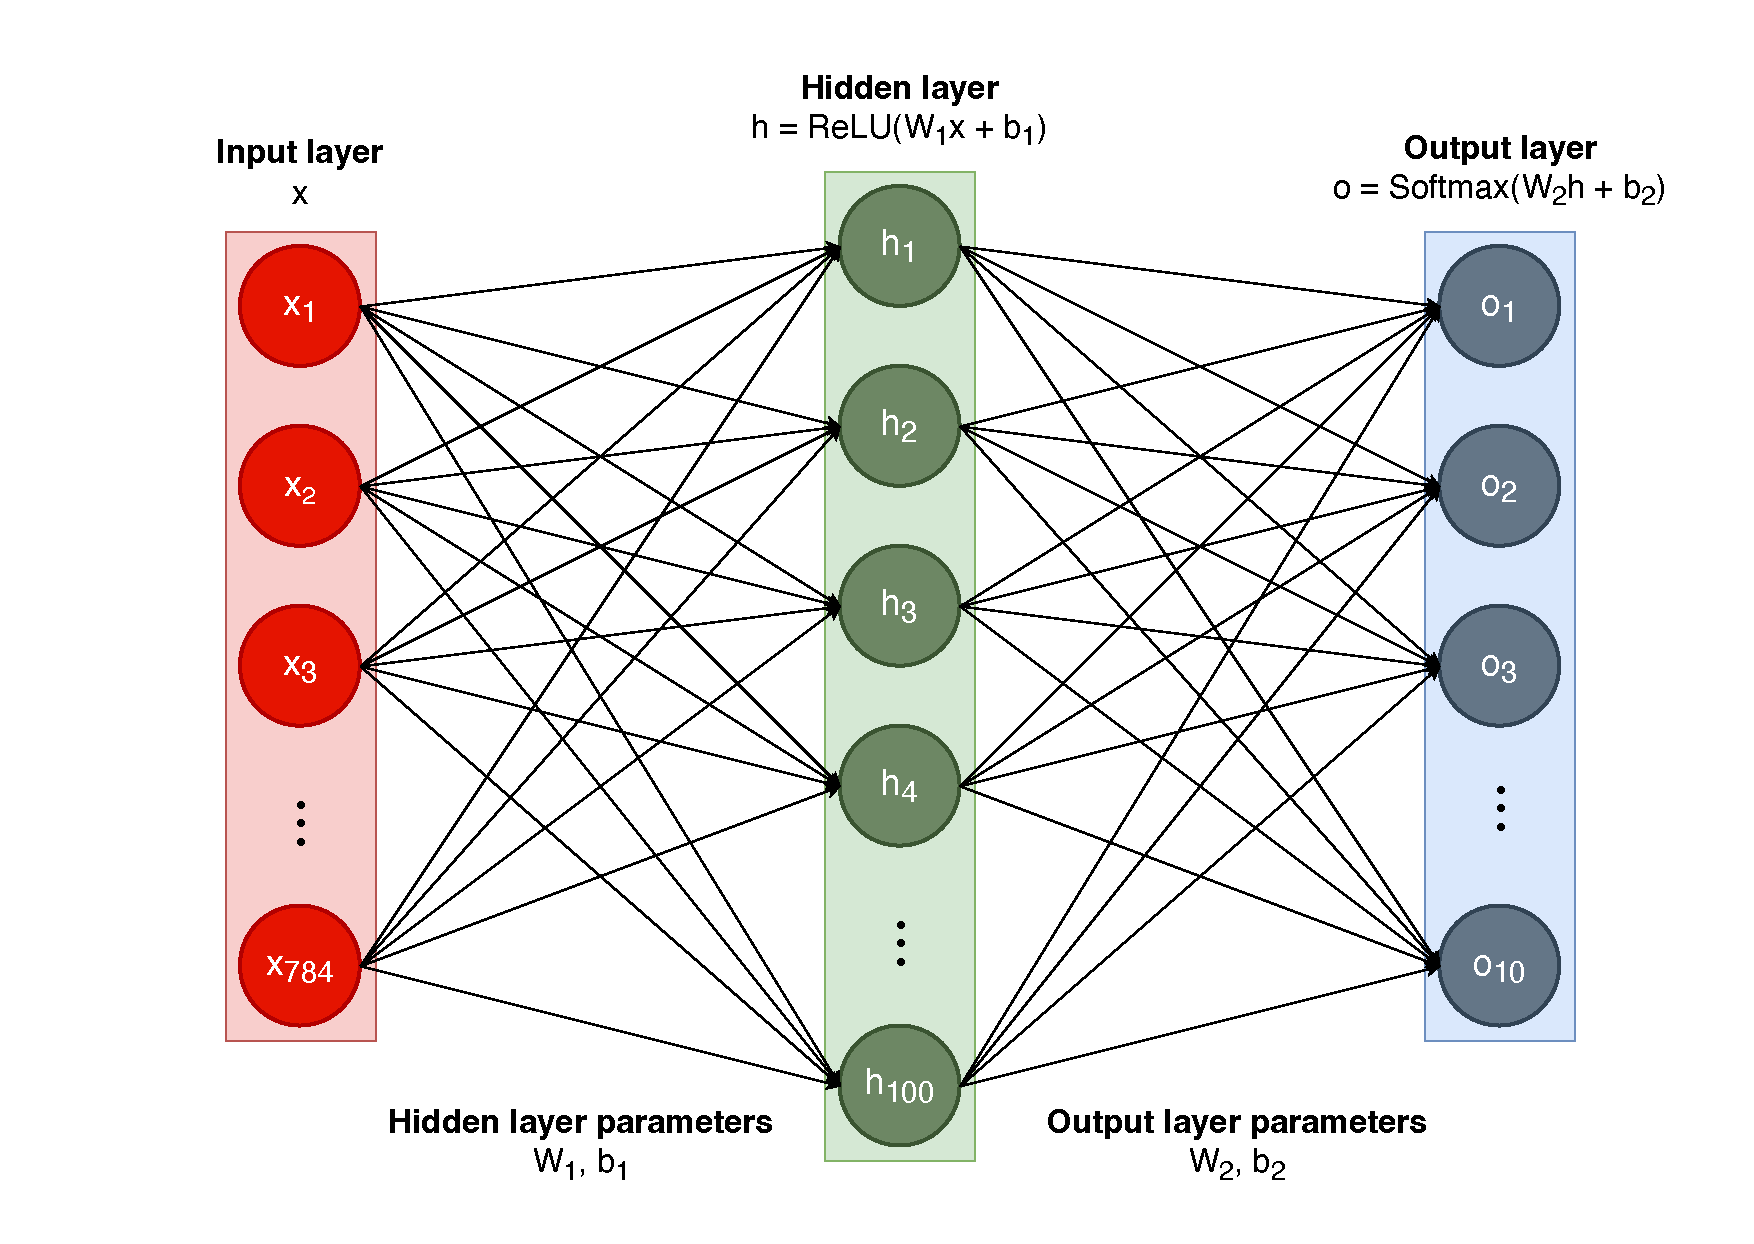
\includegraphics[width=\textwidth]{mnist_model.pdf}
  \caption{The neural network with a hidden layer and an output layer}
\label{fig:back:model}
\end{figure}

This section describes two different forms of TensorFlow DL models written in
Python.
TensorFlow provides two major version libraries, TensorFlow 1.x published in
2016 and TensorFlow 2.x published in 2019. 
DL models are significantly differ in their forms depending on which library
they use. 
On TensorFlow 1.x, neural networks are manually constructed as computational
graphs using tensor variables and operations, and the networks are lazily
executed for both their training and inference on an encapsulated environment,
called {\it session}.
%The first version is TensorFlow 1.x published in 2016.
%TensorFlow 1.x provides APIs for defining tensor variables and operations
%between them.
%Developers manually define the model structure, the model operations 
%and training process using the TensorFlow 1.x APIs.
%On TensorFlow 1.x, developers need to manually define model structures, model
%operations, and their training process using APIs for defining tensor variables
%and operations between them.
%The second version is TensorFlow 2.x published in 2019.
On the other hand, TensorFlow 2.x supports the eager execution by which all
tensor operations are executed as they occur in code. 
With the eager execution feature, developers do not need to construct
computational graphs and use encapsulated environments anymore.
%developers to use plain Python syntax to define the model
%operations and the training process.
In addition, TensorFlow 2.x integrates with the Keras library, a layer-based
deep learning model library that provides a convenient interface to construct
neural networks.
%As a result, the models written in TensorFlow 1.x and TensorFlow 2.x are
%significantly differ in their forms. 

Figure~\ref{fig:back:model} illustrates an example neural network that
classifies input images into ten categories.
In the figure, vertical bars denote vectors of layers, circles denote data of
vectors, and direct edges denote data dependencies from source to destination
in vector operations.
%The model will get an input image of 784 pixels and classify it into one of ten
%output classes.
The network consists of three layers: an input layer, an output layer, and a
hidden layer between the two layers.
Each layer stores data into a vector, and the vector of a layer mutates into a
vector of another layer via vector operations.  
In the network, the input layer has a vector of length 784, and the data in the
vector is the pixels of an input image.
The hidden layer is parametrized by the two-dimensional weight matrix $W_1$ of
size 784 $\times$ 100 and the bias vector $b_1$ of length 100.
The vector of the hidden layer is computed by first multiplying the input layer
vector $x$ with the weight matrix $W_1$, adding the bias vector $b_1$, and
finally applying the ReLU activation function that makes the result as non-zero
values.
The output layer is parametrized by the two-dimensional weight matrix $W_2$ of
size 100 $\times$ 10 and the bias vector $b_2$ of length 10.
The vector of the output layer is computed by first multiplying the hidden
layer vector $h$ with the weight matrix $W_2$, adding the bias vector $b_2$,
and finally applying the Softmax activation function that converts the ten data
as a probability distribution of the ten categories.
The weight matrices and the bias vectors in the network are model parameters,
and the training phase adjusts the model parameters again and again to classify
input images correctly.
%The model structure is defined in terms of layers and operation between them.
%The layers are tensors of real values, which represent the signals and data.
%The model in the figure \ref{fig:back:model} has three layers;
%the input layer, the hidden layer, and the output layer.
%The layers are densely connected, which means that
%the layer outputs are computed by the linear transformation with 
%the weight matrices and the bias vectors, 
%and the non-linear activation functions. 
%The hidden layer is parametrized by the weight matrix
%$W_1$ of size (784, 100) and the bias vector $b_1$ of length 100.
%The hidden layer is computed by first multiplying the input layer vector $x$
%with the weight matrix $W_1$, adding the bias vector $b_1$, and finally applying
%the ReLU activation function to the result.
%The output layer is parametrized by the weight matrix $W_2$ of size (100, 10)
%and the bias vector $b_2$ of length 10.
%The output layer is computed by first multiplying the hidden layer vector $h$
%with the weight matrix $W_2$, adding the bias vector $b_2$, and finally applying
%the Softmax activation function to the result.
%The weight matrices and the bias vectors are called the model parameters 
%as their values are updated during the training process.
%The hidden layer is a vector of length 100.
%The output layer is a vector of length 10, and each vector element represents
%the probability of the input image classified into the corresponding class.

%We describe TensorFlow 1.x and 2.x versions with code examples that define
%the same model and the same training process.
%The code examples define the neural network model illustrated
%in the figure \ref{fig:back:model}.
%The model will get an input image of 784 pixels and classify it into one of ten
%output classes.
 
%The model structure is defined in terms of layers and operation between them.
%The layers are tensors of real values, which represent the signals and data.
%The model in the figure \ref{fig:back:model} has three layers;
%the input layer, the hidden layer, and the output layer.
%The input layer is a vector of length 784, which represents the input image
%of 784 pixels.
%The hidden layer is a vector of length 100.
%The output layer is a vector of length 10, and each vector element represents 
%the probability of the input image classified into the corresponding class.
%The layers are densely connected, which means that
%the layer outputs are computed by the linear transformation with 
%the weight matrices and the bias vectors, 
%and the non-linear activation functions. 
%The hidden layer is parametrized by the weight matrix
%$W_1$ of size (784, 100) and the bias vector $b_1$ of length 100.
%The hidden layer is computed by first multiplying the input layer vector $x$
%with the weight matrix $W_1$, adding the bias vector $b_1$, and finally applying
%the ReLU activation function to the result.
%The output layer is parametrized by the weight matrix $W_2$ of size (100, 10)
%and the bias vector $b_2$ of length 10.
%The output layer is computed by first multiplying the hidden layer vector $h$
%with the weight matrix $W_2$, adding the bias vector $b_2$, and finally applying
%the Softmax activation function to the result.
%The weight matrices and the bias vectors are called the model parameters 
%as their values are updated during the training process.

The model is trained by the gradient descent algorithm. 
The gradient descent algorithm is an iterative optimization algorithm
that computes the gradients of model parameters to update their values toward
local minimum of the loss function.
The loss function defines the metric of the difference between the model 
output and answer label.
Thus, approaching the local minumum of the loss function means that the
the gradient descent trains the model to return the output similar to the
correct answer.
In DL model training, the gradient descent is repeated against several
training batches. Given a training input batch, the algorithm first computes
the model loss with forward propagation then computes the gradients of the
model parameters with backpropagation. The algorithm applies the gradients
to update the model parameters, thus approaching to the minumum loss.

\begin{figure}[ht!]
\lstinputlisting[language=Python]
{tensorflow1_mnist.py}
  \caption{TensorFlow 1.x model example}
\label{fig:back:tf1}
\end{figure}

Figure~\ref{fig:back:tf1} is a code example of a TensorFlow 1.x model.
To define a neural network model in TensorFlow 1.x, 
developers must explicitly define the model structure
and the operations between the layers. 
The developers also must manually start the training loop by explicitly
accessing the TensorFlow runtime with dedicated APIs.

First, the lines 5 to 14 define the model structure and manually build up
operaitons between the model layers.
The lines 5 and 6 first create placeholder variables {\tt x} and {\tt y},
which are the placeholders for the input image vectors 
and the answer label vectors of training data.
The placeholder variables only specify the vector size of the input images
and the labels; they will be replaced with actual values of the training
data during the training process. 
The lines 8 to 10 defines the hidden layer.
The line 8 uses the {\tt random\_uniform} API to create 
a random weight matrix of size 784 by 100, 
and the line 9 uses the {\tt zero} API to create a zero-vector of size 100.
Then, the lines 8 and 9 wrap the weight matrix and the bias vector with
{\tt Variable} API.
The {\tt Variable} API creates a TensorFlow variable that can be later modified
during the runtime. It is usually used to define a model 
parameter, whose value is changed during the training process.
Thus, the lines 8 and 9 create the weight and bias parameters for the
hidden layer which have correct sizes and are modifiable during the 
training process.
The line 10 manually defines the operations of the hidden layer. 
Note that the line does not actually compute the operations,
but only define the operations that will be computed during the training.

The lines 12 to 14 define the output layer.
Similar to the lines 8 and 9, the lines 12 and 13 define the weight matrix
and the bias vector parameter for the output layer.
Then the line 14 defines the operations of the output layer,
which multiplies the hidden layer output {\tt layer\_1} and
the weight {\tt W\_2}, adds the bias vector {\tt b\_2}, and applies the
Softmax activation function.
As shown in the lines 5 to 14, developers must explicitly define
the model components and oprations between them in TensorFlow 1.x model.

The lines 16 and 17 defines the loss function and the training operation. 
The line 16 defines the loss function between the model output {\tt layer\_2} 
and the answer label {\tt y} with categorial cross entropy function.
The line 17 defines the training operation for the model.
The line first calls the {\tt AdamOptimizer} constructor
function to create an optimizer object.
The optimizer objects in TensorFlow are abstractions of the gradient
descent algorithms.
For instance, the {\tt AdamOptimizer} abstracts a Adam gradient descent
algorithm. % todo: cite Adam g.d.
Then the {\tt minimize} method defines the training operation that updates the
TensorFlow variables via the gradient descent on the first argument.
Thus, the line 17 defines the operation of a single training step,
which optimizes the model parameters via gradient descent to the loss gradient.

The lines 19 to 22 execute the training loop. 
The line 19 first creates a {\tt Session} object.
The {\tt Session} object provides the {\tt run} method that can invoke
computation of TensorFlow operations.
The line 20 uses the {\tt run} method to initialize the TensorFlow variables.
Before the training computation starts,
the TensorFlow variables in the model and the optimizer should be initialized.
Note that the optimizer object implicitly introduces the variables which are 
used for the internal computation.
The line 20 refers to the TensorFlow global variables to initialize
all of the model parameter variables and the optimizer internal variables
at once.
After the variables are initialized, the line 21 uses the {\tt for} loop
to iterate over the dataset and get training input data. 
The number of training data is specified by the {\tt take} API of the
dataset object.
Finally, the line 22 calls the {\tt run} method to
invoke computation of the training operation {\tt train\_op}.
